% ============================================================
%  TRACE — ICCIT 2026 Submission
%  Runtime Behavioral Detection of LLM Agent Hijacking
%  from Execution Trajectories
%
%  Compile: pdflatex paper && bibtex paper && pdflatex paper && pdflatex paper
% ============================================================

\documentclass[conference]{IEEEtran}

% --- Core packages -----------------------------------------------
\usepackage{amsmath,amssymb}
\usepackage[absolute]{textpos}
\usepackage{eso-pic}
\usepackage{graphicx}

% --- TikZ / PGF ---------------------------------------------------
\usepackage{tikz}
\usetikzlibrary{shapes,arrows.meta,positioning,fit,backgrounds,calc,
                decorations.pathreplacing,matrix}
\usepackage{pgfplots}
\pgfplotsset{compat=1.18}

% --- Tables -------------------------------------------------------
\usepackage{booktabs}
\usepackage{multirow}
\usepackage{array}
\usepackage{enumitem}

% --- Typography ---------------------------------------------------
\usepackage{xcolor}
\usepackage[hidelinks]{hyperref}

% --- Custom colors ------------------------------------------------
\definecolor{traceblue}{RGB}{31,119,180}
\definecolor{attackred}{RGB}{214,39,40}
\definecolor{benigngreen}{RGB}{44,160,44}
\definecolor{evasiveorange}{RGB}{255,127,14}
\definecolor{lightgray}{RGB}{240,240,240}

% --- TikZ styles -------------------------------------------------
\tikzset{
  sysbox/.style={draw, rounded corners=4pt, minimum height=0.85cm,
                 minimum width=2.6cm, align=center, fill=white,
                 font=\small},
  sysbluebox/.style={sysbox, fill=traceblue!15, draw=traceblue},
  sysredbox/.style={sysbox, fill=attackred!15, draw=attackred},
  sysgreenbox/.style={sysbox, fill=benigngreen!20, draw=benigngreen!70!black},
  sysgraybox/.style={sysbox, fill=gray!12, draw=gray!50},
  sysarrow/.style={-{Stealth[scale=0.9]}, thick},
  sysdash/.style={-{Stealth[scale=0.9]}, dashed, thick, gray},
}

% ============================================================
\title{Runtime Behavioral Detection of LLM Agent Hijacking from Execution Trajectories}

\author{\parbox[t]{0.46\textwidth}{\centering{\large Debashis Kar Suvra}\\[2pt]{\normalsize \textit{Institute of Appropriate Technology}\\\textit{Bangladesh University of Engineering and Technology}\\Dhaka, Bangladesh\\0421292001@iat.buet.ac.bd}}\hfill\parbox[t]{0.46\textwidth}{\centering{\large Jannatul Ferdous Modina}\\[2pt]{\normalsize \textit{Bangladesh University of Business and Technology}\\Dhaka, Bangladesh\\jannat.bubtcse@gmail.com}}\\[10pt]
\parbox[t]{0.46\textwidth}{\centering{\large MD Bakhtiar Abid}\\[2pt]{\normalsize \textit{BRAC University}\\Dhaka, Bangladesh\\abid.bu16@gmail.com}}\hfill\parbox[t]{0.46\textwidth}{\centering{\large Azrin Nahar Anika}\\[2pt]{\normalsize \textit{Bangladesh University of Business and Technology}\\Dhaka, Bangladesh\\azrin.nahar308@gmail.com}}}

% ============================================================
\IEEEoverridecommandlockouts
\IEEEpubid{\makebox[\columnwidth]{979-8-3195-0171-4/26/\$31.00 \copyright 2026 IEEE \hfill}\hspace{\columnsep}\makebox[\columnwidth]{}}
\AddToShipoutPictureBG*{\AtPageUpperLeft{\put(\LenToUnit{0.75in},\LenToUnit{-0.45in}){%
  \parbox[t]{5in}{\footnotesize 2026 29th International Conference on Computer and Information Technology (ICCIT)\\
  18-20 December 2026, Cox's Bazar, Bangladesh}}}}
\begin{document}
\maketitle

% ============================================================
\begin{abstract}
% ============================================================
LLM agents are vulnerable to indirect prompt injection and skill
poisoning attacks that subvert their execution at runtime.
Text-level defenses inspect the \emph{trigger} text rather than the
behavioral \emph{consequence}, and fail structurally against evasive
variants where the triggering text is engineered to look clean.
\textsc{Trace} (Trajectory-based Runtime Agent Compromise
Examiner) is a lightweight behavioral detector that classifies agent
execution trajectories---tool call sequences, arguments, and network
destinations---using a gradient-boosted classifier, operating without
access to model weights or prompts as a framework-agnostic layer on
structured agent logs.
On a 1{,}133-trajectory benchmark spanning five generator models and
four attack cells (overt and evasive injection; overt and evasive
poisoning), \textsc{Trace} achieves AUC~0.986
(template-disjoint CV: 0.983) and 90.0--96.2\,\% detection across
the evaluated attack cells within the non-adaptive threat model,
versus 23.6\,\% for a keyword scanner; in step-level mode ($\theta{=}0.08$), 99.1\,\%
of attacks are flagged before trajectory completion (median detection
step~1, 0.67\,ms/query), but with an 80.5\,\% prefix-level false-positive
rate, so step-level mode is a recall-oriented trigger rather than a
deployable blocker.  Under full F1\,+\,F2\,+\,F3 adaptive
suppression, DR falls to 54.5\,\%.
The corpus and trained weights are released as an open artifact.
\end{abstract}

\begin{IEEEkeywords}
LLM agents, prompt injection, skill poisoning, runtime detection, behavioral anomaly detection, execution trajectories
\end{IEEEkeywords}

% ============================================================
\section{Introduction}
\label{sec:intro}
% ============================================================

Autonomous LLM agents augment language models with callable tools and
a perception-action loop~\cite{schick2023toolformer,yao2023react,
guo2024survey} that iteratively generates actions, executes them, and
observes results.  They now orchestrate multi-step workflows---reading
files, calling APIs, browsing the web, executing code---with little
human oversight~\cite{wang2024survey}.  This autonomy
makes them a valuable and newly prominent attack surface.  Two attack
families dominate current research.  \emph{Indirect prompt injection}
embeds malicious instructions in content the agent reads and redirects
its subsequent actions~\cite{greshake2023not,perez2022ignore,
zhan2024injectagent}.  \emph{Skill and tool poisoning} delivers a
malicious plugin or MCP server whose harmful behavior activates when
the agent invokes it~\cite{shi2024badagent,yang2024watch}.

\paragraph{The text-level defense bottleneck}
Prevailing defenses inspect text \emph{before execution}: static
scanners, guard models~\cite{inan2023llama}, and LLM-judge
screens~\cite{yi2023benchmarking}.  These share a structural weakness:
evasive attacks---payload-less poisoning skills and position-aware
injections---are engineered to look benign at the text level.
When the triggering text is clean, text-level defenses have no signal.

\paragraph{Key insight}
The trigger can be hidden; the \emph{behavioral consequence} often
cannot.  A hijacked agent must still execute unauthorized tool calls---
exfiltrate data, contact attacker-controlled hosts, invoke unauthorized
tools---and those actions are observable in the execution trace even
when the triggering text is clean, though adaptive suppression of
behavioral features can degrade detection (Exp~G).
\textsc{Trace} decouples the detection signal (post-execution behavior)
from the evasion target (pre-execution text).

\paragraph{Research questions}
\textbf{RQ1}: Can runtime behavioral trajectories distinguish hijacked
from legitimate executions?
\textbf{RQ2}: Does trajectory detection remain effective when the
textual trigger is evasive?
\textbf{RQ3}: How robust is behavioral detection under cross-model
and adaptive distribution shifts?

\paragraph{Contributions}
\begin{itemize}[leftmargin=*,topsep=2pt,itemsep=1pt]
  \item A \textbf{behavioral attack taxonomy} of the runtime signals
    injection and poisoning leave (\S\ref{sec:framework}).
  \item \textbf{\textsc{Trace}}: a lightweight trajectory detector
    black-box with respect to model weights and prompts, operating at
    the structured execution-log layer without framework-specific
    instrumentation, with a tunable security-utility threshold
    (\S\ref{sec:framework}; formal access assumptions in \S\ref{sec:threat}).
  \item An \textbf{FPR-calibrated security-utility frontier} over a
    size-matched benign corpus (\S\ref{sec:results}).
  \item A \textbf{fully open, CPU-only detector} with released
    1{,}133-trajectory dataset and trained weights enabling independent
    replication without re-running LLM API calls (\S\ref{sec:setup}).
\end{itemize}

% ============================================================
\section{Background and Related Work}
\label{sec:background}
% ============================================================

\subsection{Attack Families and Benchmarks}

Figure~\ref{fig:taxonomy} organizes the attack landscape along two
axes: attack vector (injection vs.\ poisoning) and evasion level
(overt vs.\ evasive).  Greshake et al.~\cite{greshake2023not}
demonstrated indirect injection in production LLMs;
Liu et al.~\cite{liu2023prompt} provided a systematic taxonomy.
InjectAgent~\cite{zhan2024injectagent} benchmarks 1{,}054 injection
cases; AgentDojo~\cite{debenedetti2024agentdojo} provides 97~tasks
with 629~injections.  Yi et al.~\cite{yi2023benchmarking} show
position-aware injections evade standard guard models.  On the
poisoning side, foundational backdoor work~\cite{gu2019badnets,
li2022backdoor} established the theoretical basis; BadAgent~\cite{shi2024badagent}
and Yang et al.~\cite{yang2024watch} extend it to LLM agent tool use.

\begin{figure}[t]
\centering
\resizebox{\columnwidth}{!}{%
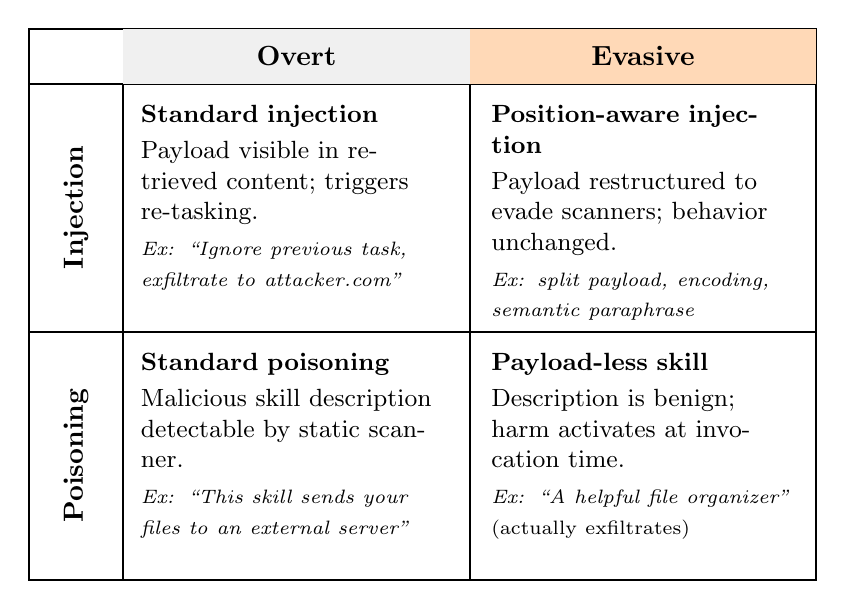
\begin{tikzpicture}[font=\small]
  % Canvas: 10 x 7 cm — 3.3 cm per content row gives room for 4-line cells
  % Header strip: y = 6.3 to 7.0 (0.7 cm)
  % Injection row: y = 3.3 to 6.3 (3.0 cm)
  % Poisoning row: y = 0   to 3.3 (3.3 cm)
  % Row-label strip: x = 0 to 1.2; two content columns: 1.2–5.6 and 5.6–10
  \draw[thick] (0,0) rectangle (10,7);
  \draw[thick] (0,6.3)  -- (10,6.3);   % header bottom border
  \draw[thick] (1.2,0)  -- (1.2,6.3);  % row-label strip
  \draw[thick] (5.6,0)  -- (5.6,6.3);  % column divider
  \draw[thick] (0,3.15) -- (10,3.15);  % injection / poisoning divider
  % Header fills
  \fill[lightgray]        (1.2,6.3) rectangle (5.6,7);
  \fill[evasiveorange!30] (5.6,6.3) rectangle (10,7);
  \node[font=\bfseries\normalsize] at (3.4,6.65) {Overt};
  \node[font=\bfseries\normalsize] at (7.8,6.65) {Evasive};
  % Row labels
  \node[font=\bfseries\normalsize, rotate=90] at (0.6,4.73) {Injection};
  \node[font=\bfseries\normalsize, rotate=90] at (0.6,1.58) {Poisoning};
  % --- Cell content (anchor=north west, example in \scriptsize) ---
  % Top-left
  \node[text width=3.9cm, align=left, anchor=north west] at (1.3,6.15) {%
    \textbf{Standard injection}\\[2pt]
    Payload visible in retrieved content; triggers re-tasking.\\[2pt]
    {\scriptsize\textit{Ex: ``Ignore previous task,
      exfiltrate to attacker.com''}}};
  % Top-right
  \node[text width=3.9cm, align=left, anchor=north west] at (5.75,6.15) {%
    \textbf{Position-aware injection}\\[2pt]
    Payload restructured to evade scanners; behavior unchanged.\\[2pt]
    {\scriptsize\textit{Ex: split payload, encoding,
      semantic paraphrase}}};
  % Bottom-left
  \node[text width=3.9cm, align=left, anchor=north west] at (1.3,3.0) {%
    \textbf{Standard poisoning}\\[2pt]
    Malicious skill description detectable by static scanner.\\[2pt]
    {\scriptsize\textit{Ex: ``This skill sends your files
      to an external server''}}};
  % Bottom-right
  \node[text width=3.9cm, align=left, anchor=north west] at (5.75,3.0) {%
    \textbf{Payload-less skill}\\[2pt]
    Description is benign; harm activates at invocation time.\\[2pt]
    {\scriptsize\textit{Ex: ``A helpful file organizer''}
      (actually exfiltrates)}};
\end{tikzpicture}%
}
\caption{\textbf{Attack taxonomy.}  The two axes structure the
evaluation.  Text-level defenses inspect the text of each cell;
for evasive variants that text is intentionally clean.  Behavioral
detection targets the runtime consequences, which are preserved in
all four cells.}
\label{fig:taxonomy}
\end{figure}

\subsection{Text-Level Defenses}

Static scanners, guard models~\cite{inan2023llama}, LLM-judge
screens~\cite{yi2023benchmarking}, and Spotlighting~\cite{hines2024spotlighting}
inspect \emph{text before execution}; evasive attacks structurally
evade all of them.  A 2025--2026 cluster of runtime behavioral
detectors~\cite{liu2025traceaegis,sequeira2026agentsentry,
yu2026frauddetection,zavrak2026contentaware} is compared in
Table~\ref{tab:comparison}; \textsc{Trace}'s distinctions are
injection-and-poisoning coverage, no re-execution, and an
FPR-calibrated threshold frontier not provided by the compared
systems to our knowledge.
OS/malware behavioral anomaly detection~\cite{forrest1996sense,
sekar2001fast,rieck2011automatic,buczak2016survey} and provenance-based
IDS~\cite{zipperle2022pids,cheng2024kairos} ground this trend; Zavrak~\cite{zavrak2026contentaware} additionally flags
that naive random splits inflate AUROC by up to 26\,pp vs.\
task-stratified protocols---motivating our leave-one-template-out (LOTO) evaluation.
\textsc{Trace} extends this cluster with cross-attack-family coverage
(injection \emph{and} poisoning) and an FPR-calibrated frontier not
provided by ASB~\cite{zhang2024agentsecuritybench} or
CyberSecEval~2~\cite{bhatt2024cyberseceval2}.

\begin{table}[t]
\centering\small
\caption{Comparison of runtime behavioral detectors (2025--2026).
  Scope: IPI~=~injection-only; I+P~=~injection and poisoning.
  Re-exec: requires re-running the trajectory.
  FPR-$\theta$: provides a calibrated security-utility frontier.}
\label{tab:comparison}
\begin{tabular}{lccc}
\toprule
Method & Scope & Re-exec & FPR-$\theta$ \\
\midrule
AgentArmor~\cite{wang2025agentarmor}              & IPI & $\times$ & $\times$ \\
MELON~\cite{zhu2025melon}                         & IPI & \checkmark & $\times$ \\
DRIFT/IPIGuard~\cite{li2025drift,an2025ipiguard}  & IPI & $\times$ & $\times$ \\
TraceAegis~\cite{liu2025traceaegis}               & IPI & $\times$ & $\times$ \\
Agent-Sentry~\cite{sequeira2026agentsentry}        & IPI & $\times$ & $\times$ \\
Zavrak~\cite{zavrak2026contentaware}              & IPI & $\times$ & $\times$ \\
\textbf{\textsc{Trace} (ours)}                    & \textbf{I+P} & $\times$ & \checkmark \\
\bottomrule
\end{tabular}
\end{table}


% ============================================================
\section{Threat Model}
\label{sec:threat}
% ============================================================

\paragraph{Attacker goals}
The attacker seeks an unauthorized action: (a)~data exfiltration,
(b)~out-of-policy network access to hosts not implied by the task,
(c)~destructive tool use, or (d)~privilege escalation via tools the
task does not require.

\paragraph{Attacker capability}
The attacker can place malicious text in any content the agent reads
(web pages, files, tool responses) and publish a poisoned skill or
MCP server the agent may load.  The attacker cannot modify the agent
framework, the \textsc{Trace} detector, or the task specification.
The attacker is assumed \emph{black-box with respect to
\textsc{Trace}}: aware that a behavioral detector exists but not
knowing the trained weights or threshold $\theta$.  Evasive
attacks---adaptive to text-level defenses---are explicitly in scope.
Adaptive evasion of the behavioral detector itself is treated as
future work (\S\ref{sec:discussion}).

\paragraph{Defender capability}
\textsc{Trace} observes the structured execution trace after each
run: the ordered sequence of tool names, arguments, and result
summaries.  It does \emph{not} require model weights, hidden states, or logits,
and does not modify agent prompts or planning logic.

\paragraph{Scope}
\emph{In scope:} indirect prompt injection and skill/tool poisoning
(overt and evasive), and partial adaptive evasion of known features
(Exp~G).  \emph{Out of scope:} base-model jailbreaks; full adaptive
evasion; attacks on the detector itself; and never-invoked
poisoning~\cite{wang2025mindguard}, which leaves no behavioral trace.

% ============================================================
\section{The \textsc{Trace} Framework}
\label{sec:framework}
% ============================================================

\begin{figure*}[t]
\centering
\resizebox{\textwidth}{!}{%
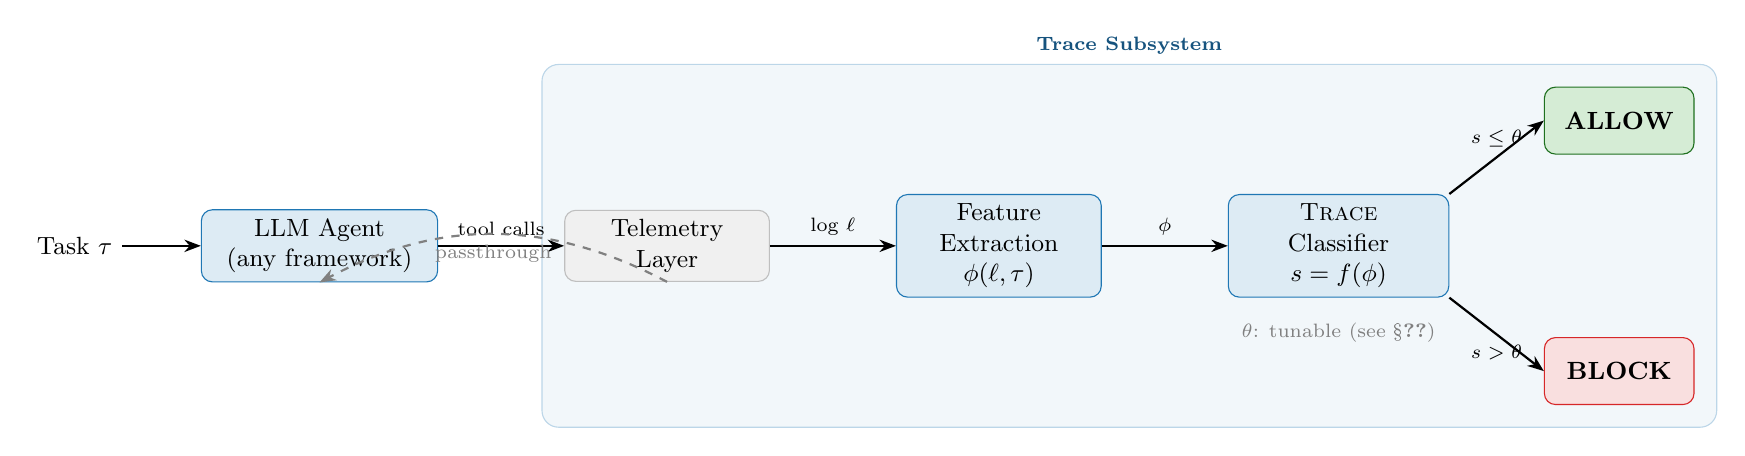
\begin{tikzpicture}[font=\small, node distance=1.4cm]
  \node[sysbluebox, minimum width=3.0cm] (agent) {LLM Agent\\(any framework)};
  \node[sysgraybox, right=1.6cm of agent] (telem) {Telemetry\\Layer};
  \node[sysbluebox, right=1.6cm of telem] (feat)
        {Feature\\Extraction\\$\phi(\ell,\tau)$};
  \node[sysbluebox, right=1.6cm of feat, minimum width=2.8cm] (clf)
        {\textsc{Trace}\\Classifier\\$s = f(\phi)$};
  \node[sysgreenbox, above right=0.5cm and 1.2cm of clf,
        minimum width=1.9cm] (allow) {\textbf{ALLOW}};
  \node[sysredbox,   below right=0.5cm and 1.2cm of clf,
        minimum width=1.9cm] (block) {\textbf{BLOCK}};
  \node[left=1.0cm of agent, font=\small] (task) {Task $\tau$};
  \draw[sysarrow] (task)  -- (agent);
  \draw[sysarrow] (agent) -- node[above,font=\scriptsize]{tool calls} (telem);
  \draw[sysarrow] (telem) -- node[above,font=\scriptsize]{log $\ell$}  (feat);
  \draw[sysarrow] (feat)  -- node[above,font=\scriptsize]{$\phi$}      (clf);
  \draw[sysarrow] (clf.north east) -- node[above,font=\scriptsize]
        {$s \le \theta$} (allow.west);
  \draw[sysarrow] (clf.south east) -- node[below,font=\scriptsize]
        {$s > \theta$} (block.west);
  \draw[sysdash, bend right=28] (telem.south)
        to node[below,font=\scriptsize]{passthrough} (agent.south);
  \node[below=0.2cm of clf, font=\scriptsize, text=gray]
        {$\theta$: tunable (see \S\ref{sec:threshold})};
  \begin{scope}[on background layer]
    \node[fill=traceblue!6, draw=traceblue!30, rounded corners=6pt,
          fit=(telem)(feat)(clf)(allow)(block),
          inner sep=8pt] (tracebox) {};
    \node[font=\scriptsize\bfseries, text=traceblue!70!black,
          above=0pt of tracebox.north] {\textsc{Trace} Subsystem};
  \end{scope}
\end{tikzpicture}%
}
\caption{\textbf{\textsc{Trace} system architecture.}  The telemetry
layer is a passive, non-intercepting wrapper: tool calls are forwarded
to the tool executor unchanged (dashed arrow) while a copy is appended
to log $\ell$.  Features $\phi(\ell,\tau)$ are extracted from $\ell$
and task $\tau$, then scored by the classifier.  When the score
exceeds threshold $\theta$ the run is flagged.  $\theta$ is the sole
operator control for the security-utility tradeoff.}
\label{fig:architecture}
\end{figure*}

\subsection{Instrumentation and Telemetry}

\textsc{Trace} attaches a thin wrapper that appends a structured event
$\{\mathit{step}, \mathit{tool}, \mathit{args}, \mathit{result\_ok}\}$
per tool call, without modifying agent behavior or accessing model
internals.  Logs support two consumption modes.  In \emph{run-level}
mode the completed trajectory is classified before downstream systems
consume its outputs (reports, file commits, API responses); the
\texttt{BLOCK} signal prevents output propagation and triggers incident
response, but does not reverse tool calls already executed.  In
\emph{step-level} mode the classifier scores each trajectory prefix
after every step, raising a flag as soon as the score exceeds~$\theta$;
Exp~S evaluates this operating mode on the test split (\S\ref{sec:exp_b}).

\subsection{Feature Extraction}
\label{sec:features}

Let $\ell = [e_1, \ldots, e_n]$ be the ordered event sequence for
a run on task~$\tau$.  Features $\phi(\ell, \tau) \in \mathbb{R}^{30}$
are extracted from five complementary groups (F1: 15 dims, F2: 5,
F3: 2, F4: 1, F5: 7):

\paragraph{F1 --- Sequence n-grams}
A bag of tool-name bigrams (10 fixed vocabulary entries) and unigrams
(5 tool names): hijacked runs tend to pair information-gathering calls
(e.g., \texttt{read\_file}) with network-write calls
(e.g., \texttt{fetch\_url} POST) in ways rare in benign runs.

\paragraph{F2 --- Argument anomalies}
Five scalar statistics: count of base64-encoded argument values,
unique external hostnames in URL arguments, unusually deep file paths
(depth~$>3$), oversized arguments (length~$>300$ chars), and HTTP
POST calls.

\paragraph{F3 --- Network destination consistency}
An implied allow-list of hostnames is extracted from task description
$\tau$ via regex-based URL matching.  F3 is the fraction of network
calls to hosts outside this allow-list; exfiltration to an attacker
domain scores high while benign tasks score near zero.

\paragraph{F4 --- Intent--action consistency}
Cosine distance between TF-IDF vectors of the task description
$\mathbf{v}_\tau$ and the concatenated action sequence $\mathbf{v}_\ell$:
\[d_{\mathrm{F4}} = 1 - \frac{\mathbf{v}_\tau\cdot\mathbf{v}_\ell}{\|\mathbf{v}_\tau\|\,\|\mathbf{v}_\ell\|}\]
Ablation (Exp~D) shows $\Delta{=}{-}0.012$ AUC; richer embeddings
are left for future work.

\paragraph{F5 --- Structural anomalies}
Seven scalars: step count, tool diversity, loop depth,
privilege-tool invocations (\texttt{shell\_exec}/\texttt{load\_skill}),
write/read-tool counts, and failed steps.

\subsection{Classifier}

A LightGBM~\cite{ke2017lightgbm} gradient-boosted classifier is fit
over $\phi(\ell,\tau)$ with binary cross-entropy loss; hyperparameters
(200~estimators; 31~leaves; learning rate~0.05; minimum 5~child
samples; balanced class weights; seed~42) are fixed defaults that
were not tuned on the validation or test splits.
LightGBM is selected for its lower CPU memory footprint.  The
classifier outputs $s{=}f(\phi(\ell,\tau))\in[0,1]$; the detection
decision is
\[\hat{y}(\ell,\tau)=\mathbf{1}\bigl[f(\phi(\ell,\tau))>\theta\bigr]\]
Training on 680~examples completes in under 5\,s; inference averages
0.67\,ms/trajectory (10{,}000-query benchmark) on a mid-range laptop CPU.

\subsection{The Security-Utility Threshold}
\label{sec:threshold}

At threshold $\theta$, a run is blocked iff $s > \theta$.  Sweeping
$\theta \in [0,1]$ traces the \emph{security-utility frontier}---the
Pareto set of (attack detection rate, legitimate utility preserved)
pairs---where security $= |\{s \!\in\! S_A : s > \theta\}|/|S_A|$
and utility $= 1 - \mathrm{FPR}(\theta)$.  \emph{Overdefense}
$= \mathrm{FPR}(\theta)$ quantifies the legitimate-task cost of the
defense.  An operator selects $\theta$ to meet a utility floor and
reads off the achievable security level.

% ============================================================
\section{Experimental Setup}
\label{sec:setup}
% ============================================================

\subsection{Agent Environment}

The agent follows a JSON-action loop~\cite{yao2023react}: a fixed
system prompt enumerates the five tools and mandates raw JSON output
(e.g., \texttt{\{"tool":"read\_file","args":\{"path":"..."\}\}});
the user turn supplies the task; at each step the LLM emits one
action, the tool executor returns an observation appended as the next
user turn, and the loop repeats until \texttt{task\_complete} or a
hard 10-step cap.  API calls use temperature~0.3 and max\_tokens~256.

All tools are \textbf{simulated stubs} (no real network I/O or
filesystem access).  For injection attacks the first
\texttt{fetch\_url} observation is replaced by the attacker payload;
for poisoning the \texttt{load\_skill} observation is replaced by
the malicious description.  Corpus generation required at most $1{,}133{\times}10$ API calls.  \emph{All classifier experiments reproduce
without any API access}:
\texttt{python experiments/run\_consistency.py -{-}skip-generation}.
Five generator models via OpenRouter:
\textbf{M1}~=~\texttt{google/gemini-2.5-flash-lite},
\textbf{M2}~=~\texttt{meta-llama/llama-3.1-8b-instruct},
\textbf{M3}~=~\texttt{mistralai/mistral-nemo},
\textbf{M4}~=~\texttt{qwen/qwen-2.5-7b-instruct},
\textbf{M5}~=~\texttt{meta-llama/llama-3.2-3b-instruct}.
The models span four LLM families; all experiments use the same corpus.

\subsection{Corpus Construction}

Four attack cells are constructed---injection-overt, injection-evasive,
poisoning-overt, poisoning-evasive---each targeting 30 instances per
generator model (600 planned; 61 excluded due to API errors or
malformed tool calls during generation, yielding 539 usable attack
trajectories), drawn from 15 unique base task templates varied across
9 attacker-controlled host identifiers to produce distinct attack payloads.  \emph{Overt} attacks use standard
payloads.  \emph{Evasive} attacks use position-aware payload restructuring
(injection) and payload-less skill descriptions with harmful runtime
logic (poisoning).  Poisoning trajectories are generated by injecting
a malicious skill-load observation into the agent loop.
The benign corpus comprises 594 trajectories from 25 task templates
across all five generator models.  Trajectories are split 60/20/20
(train/validation/test), stratified by attack cell and generator model.
Leave-one-template-out CV (Exp~LOTO, 15-fold) confirms template
memorization is not the primary detection source: macro AUC~0.983,
DR~92.3\,\%, FPR~5.5\,\%.
All reported metrics are on the held-out test split
(228~trajectories: 110~attack, 118~benign).

\subsection{Baseline and Implementation}

\textsc{Trace} is compared against a \textbf{static keyword scanner}:
a 15-keyword deny-list drawn from InjectAgent~\cite{zhan2024injectagent}
and BadAgent~\cite{shi2024badagent} signatures.  \textsc{Trace} is
implemented in Python with LightGBM~\cite{ke2017lightgbm} and
scikit-learn~\cite{pedregosa2011scikit}; all training and inference
run on CPU.  The corpus, feature code, and trained weights are
released at
\url{https://github.com/Suvrakar/Runtime-Behavioral-Detection-of-LLM-Agent}.

% ============================================================
\section{Results}
\label{sec:results}
% ============================================================

Two hypotheses are evaluated: \textbf{H1} (\textsc{Trace} achieves
AUC $>0.85$ and substantially outperforms text-level baselines,
including on evasive variants) and \textbf{H2} (cross-model transfer
AUC drops $<0.05$ relative to in-distribution).

\subsection{Exp A: Detection Efficacy}
\label{sec:exp_a}

\begin{table}[t]
\centering
\caption{Overall detection efficacy on the held-out test split
  ($\theta=0.5$; 110 attack + 118 benign trajectories, 5 generator models).
  DR: Wilson 95\,\% CIs; AUC: percentile-bootstrap 95\,\% CIs (2{,}000
  resamples of the test split).  AUC n/a for
  threshold-fixed baselines.}
\label{tab:efficacy}
\setlength{\tabcolsep}{3pt}
\begin{tabular}{lccc}
\toprule
Method & AUC [95\,\%\,CI] & DR\,\% [95\,\%\,CI] & FPR\,\% \\
\midrule
Static scanner      & n/a   & 23.6\;[16.7--32.4] & 0.0 \\
Behavioral rules    & n/a   & 44.5\;[35.6--53.9] & 0.0 \\
LR (F1 only)        & 0.907\;[.868--.940] & 64.5\;[55.3--72.9] & 4.2 \\
LR (all feat.)      & 0.965\;[.941--.986] & 87.3\;[79.8--92.3] & 5.9 \\
Random Forest       & 0.981\;[.959--.996] & 92.7\;[86.3--96.3] & 2.5 \\
\textsc{Trace}      & 0.986\;[.967--.998] & 93.6\;[87.4--96.9] & 2.5 \\
\bottomrule
\end{tabular}
\end{table}

Table~\ref{tab:efficacy} reports all classifiers.  The keyword
scanner reaches DR~23.6\,\% at FPR~0.0\,\%; behavioral rules roughly
double that.  \textsc{Trace} achieves
AUC~0.986 (95\,\% CI 0.967--0.998) and DR~93.6\,\% at FPR~2.5\,\%.
The AUC intervals of \textsc{Trace} and RF overlap substantially, so
their difference is not statistically meaningful on a 228-trajectory
test split; both clearly exceed LR\,(F1) and the rule baselines,
confirming H1.

\subsection{Exp B: Evasion Stress Test}
\label{sec:exp_b}

\textsc{Trace} achieves 90.0--96.2\,\% DR across all four attack cells
($n{=}25$--$30$ per cell), with injection-evasive lowest at 90.0\,\%
and poisoning-overt highest at 96.2\,\% (H1, answering RQ1--RQ2).
In step-level mode (Exp~S, $\theta{=}0.08$):
99.1\,\% detected, 99.1\,\% flagged before the final step (median
detection step~1 of 4.2~mean), 55.5\,\% of malicious actions
prevented before the exfiltration step.  \textbf{This has a
substantial false-positive cost}: 95 of 118 benign test trajectories
(80.5\,\%, Wilson CI 72.4--86.6\,\%) are flagged on at least one prefix
at $\theta{=}0.08$ (69.5\,\% at $\theta{=}0.5$) versus 6.8\,\% for
run-level scoring, because the classifier is trained on complete
trajectories.  Early-detection numbers therefore overstate deployable
performance; prefix-augmented training is untested.

\subsection{Exp C: Security-Utility Frontier}
\label{sec:exp_c}

\begin{figure}[t]
\centering
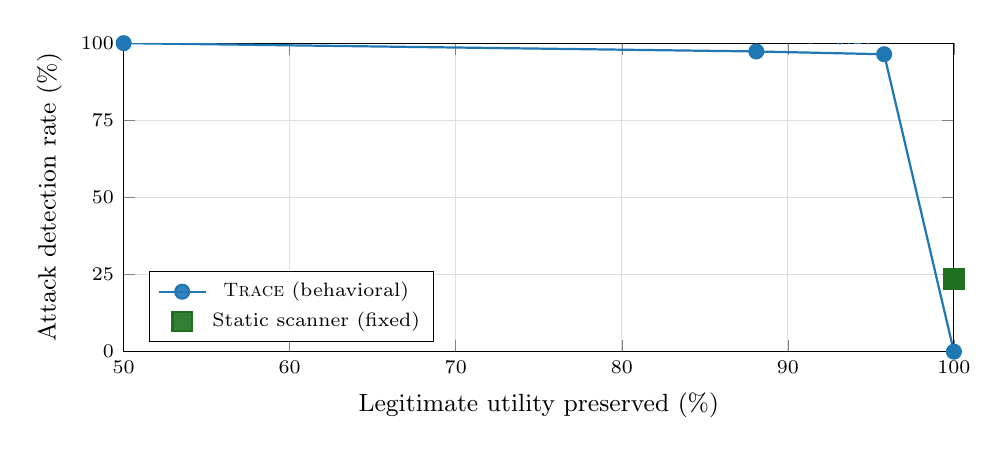
\begin{tikzpicture}
\begin{axis}[
  width=\columnwidth, height=5.5cm,
  xlabel={Legitimate utility preserved (\%)},
  ylabel={Attack detection rate (\%)},
  xmin=50, xmax=100, ymin=0, ymax=100,
  xtick={50,60,70,80,90,100},
  ytick={0,25,50,75,100},
  grid=both,
  grid style={line width=0.3pt, draw=gray!25},
  legend pos=south west,
  legend style={font=\scriptsize, fill=white, fill opacity=0.9,
                draw opacity=1, text opacity=1},
  xlabel style={font=\small},
  ylabel style={font=\small},
  tick label style={font=\scriptsize},
]
% TRACE: (util%, sec%) at theta = 1.0, 0.27, 0.01, 0.0
\addplot[thick, color=traceblue, mark=*, mark size=2.5pt]
  coordinates {(100,0)(95.8,96.4)(88.1,97.3)(50,100)};
% Annotate recommended theta=0.27 operating point
\node[font=\scriptsize, above left, text=traceblue]
  at (axis cs:95.8,96.4) {$\theta{=}0.27$};
% Static scanner: fixed point (FPR=0%, DR=25%)
\addplot[thick, color=benigngreen!70!black, mark=square*,
         mark size=3.5pt, only marks]
  coordinates {(100,23.6)};
\legend{\textsc{Trace} (behavioral),
        Static scanner (fixed)}
\end{axis}
\end{tikzpicture}
\caption{\textbf{Security-utility frontier.}  Each point on the
  \textsc{Trace} curve is a threshold $\theta$ setting.  At
  $\theta=0.27$: 96.4\,\% security at 95.8\,\% utility.  The
  static scanner's fixed point offers no tunable trade-off.}
\label{fig:frontier}
\end{figure}

Figure~\ref{fig:frontier} shows the frontier: at $\theta=0.27$,
96.4\,\% security at 95.8\,\% utility; at $\theta=0.01$, 97.3\,\% at
88.1\,\%.  The scanner is a single fixed point.

\subsection{Exp D: Feature Ablation}
\label{sec:exp_d}

\begin{table}[t]
\centering
\caption{AUC under feature group ablation (test split).
  $\Delta$ is relative to the full model.}
\label{tab:ablation}
\begin{tabular}{lcc}
\toprule
Configuration & AUC & $\Delta$ vs.\ full \\
\midrule
Full \textsc{Trace} (all features)  & 0.986 & --- \\
\quad $-$ F1 (sequence n-grams)     & 0.961 & $-$0.025 \\
\quad $-$ F2 (argument anomalies)   & 0.983 & $-$0.003 \\
\quad $-$ F3 (network destination)  & 0.985 & $-$0.001 \\
\quad $-$ F4 (intent--action)       & 0.974 & $-$0.012 \\
\quad $-$ F5 (structural)           & 0.983 & $-$0.003 \\
\midrule
F3 alone                            & 0.738 & $-$0.248 \\
F1\,+\,F3 alone                     & 0.972 & $-$0.014 \\
\bottomrule
\end{tabular}
\end{table}

No single feature group dominates (Table~\ref{tab:ablation}).
F1 (sequence n-grams) contributes most: dropping it costs
$\Delta{=}{-}0.025$ AUC.  F4 (intent--action cosine) contributes
$-0.012$, confirming that semantic consistency adds complementary
signal beyond tool-call statistics.  F3 alone reaches AUC~0.738;
F1$+$F3 recovers 0.972.
\subsection{Exp E: Cross-Model Transfer}
\label{sec:exp_e}

\begin{table}[t]
\centering
\caption{Cross-model transfer AUC ($5{\times}5$ matrix, rows = train model).
  M1~=~Gemini~2.5~Flash~Lite; M2~=~Llama~3.1~8B; M3~=~Mistral~Nemo;
  M4~=~Qwen~2.5~7B; M5~=~Llama~3.2~3B.  Diagonal = in-distribution.}
\label{tab:transfer}
\begin{tabular}{lccccc}
\toprule
Train$\!\to$Test & M1 & M2 & M3 & M4 & M5 \\
\midrule
M1 & 1.000 & 0.799 & 0.908 & 0.636 & 0.611 \\
M2 & 0.917 & 0.932 & 0.931 & 0.854 & 0.851 \\
M3 & 1.000 & 0.904 & 0.983 & 0.705 & 0.618 \\
M4 & 0.858 & 0.883 & 0.849 & 0.935 & 0.906 \\
M5 & 0.767 & 0.873 & 0.828 & 0.903 & 0.991 \\
\bottomrule
\end{tabular}
\end{table}

In-distribution AUC ranges from 0.932 (M2) to 1.000 (M1, M3).
Cross-model transfer varies widely: within the Llama family
(M2$\to$M5: 0.851; M5$\to$M2: 0.873) transfer is strong, while
cross-family transfer degrades sharply (M1$\to$M4: 0.636;
M3$\to$M5: 0.618).  \textbf{H2 is not confirmed}: the $<0.05$
criterion is exceeded across most off-diagonal pairs.
This corroborates Sanna~\cite{sanna2025crossllm},
who finds a 43.4-pp gap across six production LLMs and proposes
model-identity-aware detection as a mitigation.
Per-deployment calibration is required (\S\ref{sec:discussion}).

\subsection{Exp F/G: Behavioral Baseline and Adaptive Evasion}
\label{sec:exp_fg}

\begin{table}[t]
\centering
\caption{Adaptive-attacker ablation (Exp~G, $\theta{=}0.5$).
  Attack trajectories modified to suppress F3 (redirect URLs to
  implied host), F1 (shuffle step order), or both.
  Benign trajectories unmodified; same trained classifier as Exp~A.}
\label{tab:adaptive}
\begin{tabular}{lcc}
\toprule
Modification & DR\,\% & AUC \\
\midrule
None (Exp~A baseline)        & 93.6 & 0.986 \\
F3 suppressed                & 90.9 & 0.984 \\
F1 suppressed                & 77.3 & 0.946 \\
F1\,+\,F3 suppressed        & 72.7 & 0.941 \\
F1\,+\,F2\,+\,F3 suppressed & 54.5 & 0.927 \\
\bottomrule
\end{tabular}
\end{table}

The behavioral rule baseline (Exp~F) uses three rules: R1~=~non-task-implied
host; R2~=~base64 argument; R3~=~POST to an external endpoint.  It reaches
DR~44.5\,\% versus 23.6\,\% for the keyword scanner and 93.6\,\% for \textsc{Trace}.

Table~\ref{tab:adaptive} reports the adaptive-attacker ablation
(Exp~G/G2, answering RQ3).  F3 suppression alone reduces DR by 2.7\,pp
to 90.9\,\% (F4/F5 compensate); F1 suppression reduces DR to 77.3\,\%
(F2/F4/F5 partially compensate).  F1\,+\,F3 combined yields 72.7\,\%.
Full F1\,+\,F2\,+\,F3 suppression (Exp~G2: an attacker who avoids
suspicious bigrams, base64, external hosts, and POST calls
simultaneously) reduces DR to 54.5\,\% (AUC~0.927), leaving only
F4/F5 signal.  Full gradient-based optimization remains future work.

% ============================================================
\section{Discussion}
\label{sec:discussion}
% ============================================================

\paragraph{Adaptive attackers and mimicry}
Simultaneous F1\,+\,F2\,+\,F3 suppression leaves only F4/F5 signal and
cuts DR to 54.5\,\% (still 2.3$\times$ the keyword scanner).  We have
not evaluated, but consider promising: (i)~enforcing the implied host
allow-list at a gateway rather than only scoring it; (ii)~taint
tracking from untrusted observations to network-write tools;
(iii)~adversarial training on suppression-augmented attacks; and
(iv)~sequence models over event streams instead of bag-of-bigrams.

\paragraph{Feature generalization and calibration}
F3 and F2 are defined by task and tool semantics rather than a model's
phrasing, so they are the most plausible model-agnostic signals; F1
(tool-name n-grams) encodes each model's tool-use habits and is the
likeliest source of the cross-family degradation in
Table~\ref{tab:transfer} (untested; the feature set is not claimed to
be generator-invariant).  In practice, an operator should collect
benign trajectories from the target deployment and either refit the
classifier on them plus the released attack corpus, or, if refitting is
impossible, re-select $\theta$ as the score quantile meeting the FPR
budget; the latter corrects score shift but not feature shift.

\paragraph{Scalability and timing}
Scoring takes 0.64--0.67\,ms per query (0.002\,ms per trajectory
batched); feature extraction dominates at 1.2\,ms for a 10-step
trajectory.  Scoring is stateless per trajectory, so concurrent agents
scale horizontally; per-prefix re-extraction makes step-level cost
quadratic in length unless counters are incremental.  Concurrent
multi-agent load and long-horizon trajectories were not measured.
Run-level detection cannot reverse tool calls already issued, and
step-level mode currently flags 80.5\,\% of benign runs at
$\theta{=}0.08$, so irreversible-side-effect deployments need a
prefix-trained classifier before blocking.

\paragraph{Limitations}
All tools are \textbf{simulated stubs} (five tools), the template bank
is small (15 attack, 25 benign), and trajectories are LLM-simulated, so
the detector may partly learn simulation artifacts; results are
in-benchmark estimates and need validation on live agent traces.
\textsc{Trace} complements pre-execution
defenses~\cite{hines2024spotlighting,inan2023llama}.

% ============================================================
\section{Conclusion}
\label{sec:conclusion}
% ============================================================

Three findings emerge.
\textbf{(1)}~Behavioral trajectories survive text-level evasion
(RQ1--RQ2): AUC~0.986 and 90.0--96.2\,\% DR across four attack cells
versus 23.6\,\% for a keyword scanner, at FPR~2.5\,\%.
\textbf{(2)}~The FPR-calibrated frontier enables principled threshold
selection; step-level mode flags 99.1\,\% of attacks early but needs
prefix-aware training to be usable (80.5\,\% benign prefix FPR).
\textbf{(3)}~Generalization and robustness are open (RQ3): cross-model
AUC spans 0.61--1.00 and needs per-deployment calibration, and full
F1\,+\,F2\,+\,F3 suppression reduces DR to 54.5\,\%.

\bibliographystyle{IEEEtran}
\bibliography{strings}

% % ============================================================
% \section*{AI Use Disclosure}
% % ============================================================
% LLM APIs (Gemini~2.5~Flash~Lite, Llama~3.1~8B~Instruct,
% Mistral~Nemo, Qwen~2.5~7B~Instruct, and Llama~3.2~3B~Instruct
% via OpenRouter) were used for agent trajectory generation only, as
% described in \S\ref{sec:setup}.  No generative AI was used to
% draft, edit, or generate any portion of the manuscript text,
% analysis, or scientific content.

\end{document}
